%%FRAGEN:
%MIT GAIN; NOISE AMPLITUDE, ATTENUATOR RECHNEN?
%FIT UND PARAMETER EXTREM NAH AN GLEICHRICHTER??
\subsection[]{Verifikation der Funktionsweise eines Lock-in Verstärkers}
Wie in Schaltplan \textbf{PLAN REFERENZIEREN!!!} dargestellt wird über den Noise Generator ein Rauschsignal hinzu gegeben.
Das Signal ist von der gleichen Größenordnung wie die Signalspannung $U_\text{sig}$.
Analog zu Abschnitt \ref{sec:gleichrichter} werden alle Messungen wiederholt, erst ohne und dann mit Noise Generator.
Der Gain Regulierer am Verstärker ist nun auf $5$ gestellt, die Noise Amplitude und der Noise Attenuator auf $10^{-3}$.
%FRAGE: MUSS MAN DAMIT RECHEN?
Für die Messreihe ohne Integration durch den Tiefpass ergeben sich die Spannungsverlüfe \ref{fig:phasenunterschiede_mit_noise}.
%
%
\begin{figure}%
    \begin{subfigure}{0.5\textwidth}%
    \centering%
    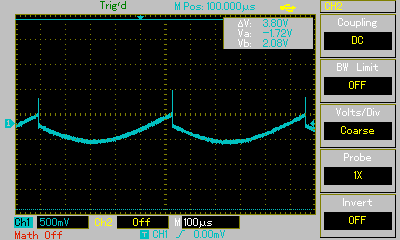
\includegraphics[width = 7.3cm]{./Oszilloskop Bilder/png/5.3/n1.png}%
    \caption{$\phi = \qty[]{0}{\degree}$}%
    \label{fig:phase6}%
    \end{subfigure}%
    %
    \hfill% Fills available space in the center -> space between figures
    \begin{subfigure}{0.5\textwidth}%
    \centering%
    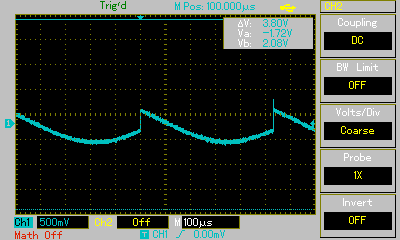
\includegraphics[width = 7.3cm]{./Oszilloskop Bilder/png/5.3/n2.png}%
    \caption{$\phi = \qty[]{45}{\degree}$}%
    \label{fig:phase7}%
    \end{subfigure}%
    %
    \hfill
    \begin{subfigure}{0.5\textwidth}%
    \centering%
    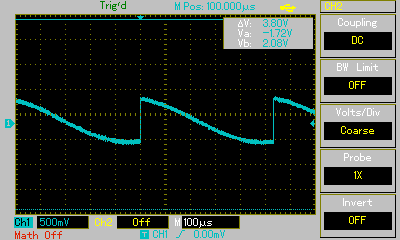
\includegraphics[width = 7.3cm]{./Oszilloskop Bilder/png/5.3/n3.png}%
    \caption{$\phi = \qty[]{90}{\degree}$}%
    \label{fig:phase8}%
    \end{subfigure}%
    %
    \hfill% Fills available space in the center -> space between figures
    \begin{subfigure}{0.5\textwidth}%
    \centering%
    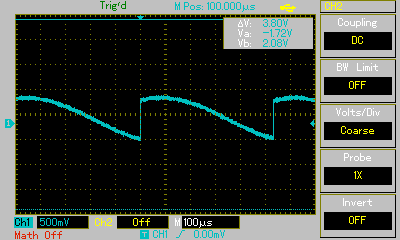
\includegraphics[width = 7.3cm]{./Oszilloskop Bilder/png/5.3/n4.png}%
    \caption{$\phi = \qty[]{135}{\degree}$}%
    \label{fig:phase9}%
    \end{subfigure}%
    %
    \hfill
    \begin{subfigure}{0.5\textwidth}%
    \centering%
    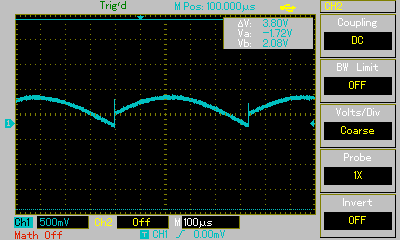
\includegraphics[width = 7.3cm]{./Oszilloskop Bilder/png/5.3/n5.png}%
    \caption{$\phi = \qty[]{180}{\degree}$}%
    \label{fig:phase10}%
    \end{subfigure}%
    %
    \caption{Spannungsverläufe für unterschiedliche Phasen ohne Integration mit Noise Generator}%
    \label{fig:phasenunterschiede_mit_noise}%
\end{figure}%

\noindent
Unter Verwendung des Tiefpasses ergeben sich abhängig von der Phasenverschiebungen $\phi$ die Spannungen
$U_\text{noise}$ in \ref{tab:u_noise}.
%
\begin{table}
    \centering
    \caption[]{Ausgangsspannung nach Integration mit Geräuschsignal}
    \label{tab:u_noise}
    \sisetup{table-format=3.0}
    \begin{tabular}[]{S c S[table-format=2.2]}
        \toprule
        {$\phi / \unit[]{\degree}$} & {$\phi / \unit[]{\radian}$} & {$U_\text{noise} / \unit[]{\volt}$} \\
        \midrule
           0 &     0          & -0.18 \\ % Ch1 Ampl in V: 1.11
          45 & $    \pi / 4 $ & -0.16 \\ % Ch1 Ampl in V: 0.7722
          90 & $    \pi / 2 $ &  0.00 \\ % Ch1 Ampl in V: 0.9306
         135 & $ 3  \pi / 4 $ &  0.22 \\ % Ch1 Ampl in V: 0.8910
         180 & $    \pi     $ &  0.34 \\ % Ch1 Ampl in V: 0.6138
         225 & $ 5  \pi / 4 $ &  0.32 \\ % Ch1 Ampl in V: 0.9306
         270 & $ 3  \pi / 2 $ &  0.16 \\ % Ch1 Ampl in V: 1.33
         300 & $ 5  \pi / 3 $ &  0.04 \\ % Ch1 Ampl in V: 1.49
         315 & $ 7  \pi / 4 $ & -0.04 \\ % Ch1 Ampl in V: 1.45
         330 & $ 11 \pi / 6 $ & -0.12 \\ % Ch1 Ampl in V: 1.21
        \bottomrule
    \end{tabular}
\end{table} 
Analog zu Abschnitt \ref{sec:gleichrichter} ergeben sich mit der Ausgleichsfunktion \eqref{eq:ausgleich_tp_ohne_noise} die Parameter
\begin{align*}
    A_\text{noise} &= \left(\num[]{-0.2747} \pm \num[]{0.0055}\right) \, \unit{\volt} & B_\text{noise} &=  \num[]{0.9933} \pm \num[]{0.0150} \\
    C_\text{noise} &= \num[]{-0.2754} \pm \num[]{0.0564} & D_\text{noise} &= \left(\num[]{0.0810} \pm \num[]{0.0054}\right) \, \unit[]{\volt},
\end{align*}
%param_a = ufloat(-0.27466768, 0.00545352)
%param_b = ufloat(0.99333910 , 0.01503098)
%param_c = ufloat(-0.27544268, 0.05641517)
%param_d = ufloat(0.08103079 , 0.00536591)

%Siganlveränderungen beschreiben!!!
